
\de{ĐỀ THI GIỮA HỌC KỲ I NĂM HỌC 2023-2024}{THPT Nguyễn Hữu Cảnh}

%Câu 1...........................
\begin{bt}%[0D1H1-3]%[Dự án đề kiểm tra Toán 10 GHKI NH23-24 - Lê Hùng Thắng]%[THPT Nguyễn Hữu Cảnh - HCM]
	Lập mệnh đề phủ định của các mệnh đề sau
	\begin{listEX}[1]
		\item $P\colon``\forall x \in \mathbb{R}, x^2>1$''.
		\item $Q\colon``\exists x \in \mathbb{R}, (2x+1)$ là số chia hết cho $3$''.
	\end{listEX}
	\loigiai{Ta có
		\begin{listEX}[1]
			\item $\overline{P}\colon``\exists x \in \mathbb{R}, x^2\leq 1$''.
			\item $\overline{Q}\colon``\forall  x \in \mathbb{R}, (2x+1)$ là số không chia hết cho $3$''.
		\end{listEX}
	}
\end{bt}

\begin{bt}%[0D1H2-1]%[Dự án đề kiểm tra Toán 10 GHKI NH23-24 - Lê Hùng Thắng]%[THPT Nguyễn Hữu Cảnh - HCM]
	Viết lại tập hợp $A$ bằng cách liệt kê các phân tử, biết
	
	$A=\left\{x \in \mathbb{Z} \mid\left(5 x-3 x^2\right) \cdot\left(x^2+2 x-3\right)=0\right\}$.
	\loigiai{
		Ta có $A=\left\{0;\, 1;\, 3\right\}$.
	}
\end{bt}

\begin{bt}%[0D1H2-2]%[Dự án đề kiểm tra Toán 10 GHKI NH23-24 - Lê Hùng Thắng]%[THPT Nguyễn Hữu Cảnh - HCM]
	Tìm tất cả các tập con gồm hai phần tử của tập hợp $B=\{a ; b ; c ; d\}$.
	\loigiai{
		Các tập con của $B$ gồm có hai phần tử là
		$\{a;b\}$, $\{a;c\}$, $\{a;d\}$, $\{b;c\}$, $\{ b,d\}$, $\{c,d\}$.
	}
\end{bt}

\begin{bt}%[0D1H3-2]%[Dự án đề kiểm tra Toán 10 GHKI NH23-24 - Lê Hùng Thắng]%[THPT Nguyễn Hữu Cảnh - HCM]
	Cho $A=\{1 ; 2 ; 3 ; 4\}$, $B=\{0 ; 1 ; 2 ; 5 ; 6\}$. Xác định $A \cap B$, $A \cup B$, $A \setminus  B$, $B \setminus  A$.
	\loigiai{
		Ta có 
		
		$A \cap B = \{1;2\}$, 
		
		$A \cup B = \{0;1;2;3;4;5;6\}$, 
		
		$A \setminus  B = \{3;4\}$, 
		
		$B \setminus  A = \{0;5;6\}$.
	}
\end{bt}

\begin{bt}%[0D1H3-4]%[Dự án đề kiểm tra Toán 10 GHKI NH23-24 - Lê Hùng Thắng]%[THPT Nguyễn Hữu Cảnh - HCM]
	Cho $A=(-5;5]$, $B=[0;7]$. Xác định $A \cap B$, $A \cup B$, $A \setminus  B$, $\mathrm{C}_{\mathbb{R}} A$.
	\loigiai{
		Ta có
		
		$A \cap B= [0;5]$,
		
		$A \cup B =(-5;7]$, 
		
		$A \setminus B=(-5;0)$, 
		
		$\mathrm{C}_{\mathbb{R}} A=\mathbb{R}\setminus A = (-\infty;-5] \cup (5;+\infty)$.	
	}
\end{bt}

\begin{bt}%[0D2Y1-2]%[Dự án đề kiểm tra Toán 10 GHKI NH23-24- Trương Quang Phú ]%[THPT Nguyễn Hữu Cảnh ]
Trên mặt phẳng tọa độ $Oxy$, hãy biểu diễn miền nghiệm của bất phương trình $3x+y-1\leq 0$.
\loigiai{
Dựng đường thẳng $\Delta\colon 3x+y-1=0$ trên mặt phẳng tọa độ.\\
Lấy tọa độ điểm $O(0,0)$ thế vào bất phương trình ta thấy điểm $O$ thuộc miền nghiệm của bất phương trình.\\
Miền nghiệm của bất phương trình là phần không bị gạch chéo trên hình vẽ. 
\begin{center}\begin{tikzpicture}[>=stealth,x=1cm,y=1cm,scale=0.8]
	\draw[->] (-4,0)--(1/3,0)node[below]{$\frac{1}{3}$}--(4,0)node[below right]{$x$};
	\draw[->] (0,-4)--(0,1)node[right]{$1$}--(0,4) node[left]{$y$};
	\draw (0,0)node[below left]{$O$};
	\path[pattern=north west lines] (-1,4)-|(4,-4)--(1.67,-4)--cycle;
	\draw (-1,4)--(1.67,-4);
	\fill (0,1)circle (1.5pt) (1/3,0)circle (1.5pt);
\end{tikzpicture}\end{center}
}
\end{bt}
\begin{bt}%[0D2K2-3]%[Dự án đề kiểm tra Toán 10 GHKI NH23-24- Trương Quang Phú ]%[THPT Nguyễn Hữu Cảnh ]
Một hộ nông dân định trồng hoa lan và hoa hồng trên diện tích $800 \mathrm{m}^2$. Nếu trồng hoa lan thì cần $20$ công và thu $3$ triệu đồng trên $100 \mathrm{m}^2$; nếu trồng hoa hồng thì cần $30$ công và thu $4$ triệu đồng trên $100\mathrm{m}^2$. Hỏi cần trồng mỗi loại hoa trên diện tích bao nhiêu để thu được nhiều tiền nhất khi tổng số công không vượt quá $180$.
\loigiai{
Gọi $x$ và $y$ lần lượt là diện tích đất trồng hoa lan và hoa hồng.\\
Tổng diện tích đất trồng hoa là $800 \mathrm{m}^2$ nên $x+y=800$.\\
Do tổng số công không vượt quá $180$ nên $20\cdot\dfrac{x}{100}+30\cdot\dfrac{y}{100}\leq 180\Leftrightarrow 2x+3y\leq 1800$.\\
Số tiền thu được là $T=3\cdot\dfrac{x}{100}+4\cdot\dfrac{y}{100}=\dfrac{3x+4y}{100}$ (triệu đồng).\\
Ta có $\dfrac{3x+4y}{100}=\dfrac{x+y}{100}+\dfrac{2x+3y}{100}\leq \dfrac{800}{100}+\dfrac{1800}{100}=26$.\\
Vậy số tiền thu được nhiều nhất là $T=26$ triệu đồng đạt được khi $$\heva{&x+y=800\\&2x+3y=1800}\Leftrightarrow\heva{&x=600\\&y=200.}$$
}
\end{bt}
\begin{bt}%[0H1B3-1]%[Dự án đề kiểm tra Toán 10 GHKI NH23-24- Trương Quang Phú ]%[THPT Nguyễn Hữu Cảnh ]
\begin{enumerate}[a)]
	\item Cho $\Delta ABC$ có $BC=10$, $\widehat{A}=45^\circ$, $\widehat{B}=60^\circ$. Tính độ dài cạnh $AC$ và bán kính đường tròn ngoại tiếp $\Delta ABC$.
	\item Cho $\Delta ABC$ có $AB=5$, $BC=3$, $CA=4$. Tính giá trị $\cos A$ và độ dài đường trung tuyến $BM$ của $\Delta ABC$.
\end{enumerate}
	\loigiai{
\begin{enumerate}[a)]
	\item 
	Áp dụng định lí sin ta có $\dfrac{BC}{\sin A}=\dfrac{AC}{\sin B}\Leftrightarrow AC=BC\cdot \dfrac{\sin A}{\sin B}=\dfrac{10\sqrt{6}}{3}$.\\
	Ta có $R=\dfrac{BC}{2\sin A}=5\sqrt{2}$.
	\item Áp dụng định lí cosin ta có $\cos A=\dfrac{AB^2+AC^2-BC^2}{2AB\cdot AC}=\dfrac{4}{5}$.\\
	Ta có $BM^2=AB^2+AM^2-2\cdot AB\cdot AM\cos \widehat{BAC}=13\Rightarrow BM=\sqrt{13}$.
\end{enumerate}	
}
\end{bt}
\begin{bt}%[0H1G3-1] %[Dự án đề kiểm tra Toán 10 GHKI NH23-24- Trương Quang Phú ]%[THPT Nguyễn Hữu Cảnh ]
Cho $\triangle ABC$ thỏa hệ thức $\sin A=\dfrac{\sin B+\sin C}{\cos B+\cos C}$. Chứng minh tam giác $ABC$ vuông.
\loigiai{
$$\sin A=\dfrac{\sin B+\sin C}{\cos B+\cos C}\Leftrightarrow \dfrac{a}{2R}=\dfrac{\dfrac{b}{2R}+\dfrac{c}{2R}}{\dfrac{a^2+c^2-b^2}{2ac}+\dfrac{a^2+b^2-c^2}{2ab}}$$
$$a=\dfrac{2abc(b+c)}{b(a^2+c^2-b^2)+(a^2+b^2-c^2)c}\Leftrightarrow (b+c)(a^2-b^2-c^2)=0\Leftrightarrow a^2=b^2+c^2 \text{ (do $b$, $c$ dương)}$$
Vậy tam giác $ABC$ vuông tại $A$.
}
\end{bt}
\begin{bt} %[0H1K3-2] %[Dự án đề kiểm tra Toán 10 GHKI NH23-24- Trương Quang Phú ]%[THPT Nguyễn Hữu Cảnh ]
Trên nóc một tôa nhà có một côt cờ cao $2 \mathrm{m}$. Từ vị trí quan sát $A$ cao $5 \mathrm{m}$ so với mặt đất, có thể nhin thấy đỉnh $B$ và chân $C$ của cột cờ dưới góc $45^{\circ}$ vâ $40^{\circ}$ so với phương nằm ngang. Tìm chiều cao của tòa nhà (làm tròn kết quả đển hàng phần mười).
\loigiai{
\immini{
Ta có $\widehat{BFK}=45^{\circ}$ và $\widehat{CFK}=40^{\circ}$. Suy ra $\widehat{BFC}=5^{\circ}$ và $\widehat{KBF}=45^{\circ}$.\\
Áp dụng định lí sin ta có $\dfrac{CF}{\sin 45^{\circ}}=\dfrac{BC}{\sin 5^{\circ}}\Leftrightarrow CF=BC\dfrac{\sin 45^\circ}{\sin 5^\circ}$\\

Suy ra $CK=CF\sin \widehat{CFK}=BC\dfrac{\sin 45^\circ}{\sin 5^\circ}\sin 40^\circ=10{,}43 \mathrm{m}$.\\
Vậy chiều cao của tòa nhà là $L=AK+KC=15{,}43 \mathrm{m}$.

}{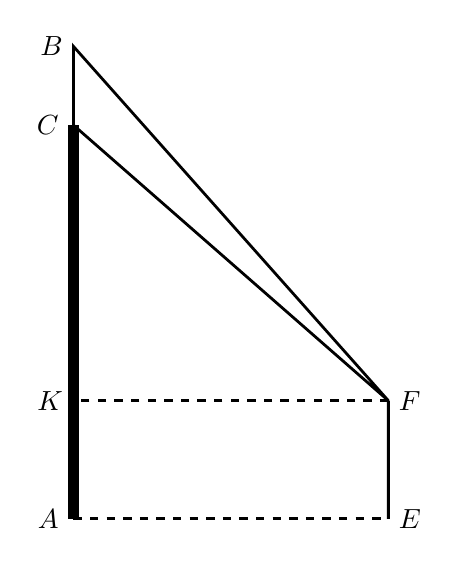
\begin{tikzpicture}
\draw[line width=4pt] (-2,0)node[left]{$A$}--(-2,5)node[left]{$C$};
\draw[line width=1pt]  (-2,5)--(-2,6)node[left]{$B$}--(2,1.5)--(-2,5) (2,0)node[right]{$E$}--(2,1.5)node[right]{$F$};
\draw[dashed, line width=1pt] (-2,0)--(2,0) (2,1.5)--(-2,1.5)node[left]{$K$};
\end{tikzpicture}}


 }
\end{bt}
